\documentclass[tikz,border=2pt,11pt]{standalone}
\usetikzlibrary{arrows.meta}
\usepackage{amsmath}
\usepackage{amssymb}
\usepackage{mathrsfs}
\usepackage{xcolor}
\usepackage{tikz}
\newcommand{\E}{\mathbb E}
\newcommand{\PP}{\mathbb P}
\newcommand{\R}{\mathbb R}
\newcommand{\Z}{\mathbb Z}
\newcommand{\N}{\mathbb N}
\newcommand{\F}{\mathcal F}
\newcommand{\Bcal}{\mathcal B}
\newcommand{\1}{\mathbf 1}
\newcommand{\dd}{\mathrm d}
\newcommand{\eps}{\varepsilon}
\newcommand{\norm}[1]{\left\lVert#1\right\rVert}
\newcommand{\abs}[1]{\left\lvert#1\right\rvert}
\newcommand{\clip}[2]{\left[#1\right]_{#2}}
\DeclareMathOperator{\dist}{dist}
\DeclareMathOperator{\diam}{diam}
\DeclareMathOperator{\supp}{supp}
\DeclareMathOperator{\Var}{Var}
\DeclareMathOperator{\TV}{TV}
\begin{document}
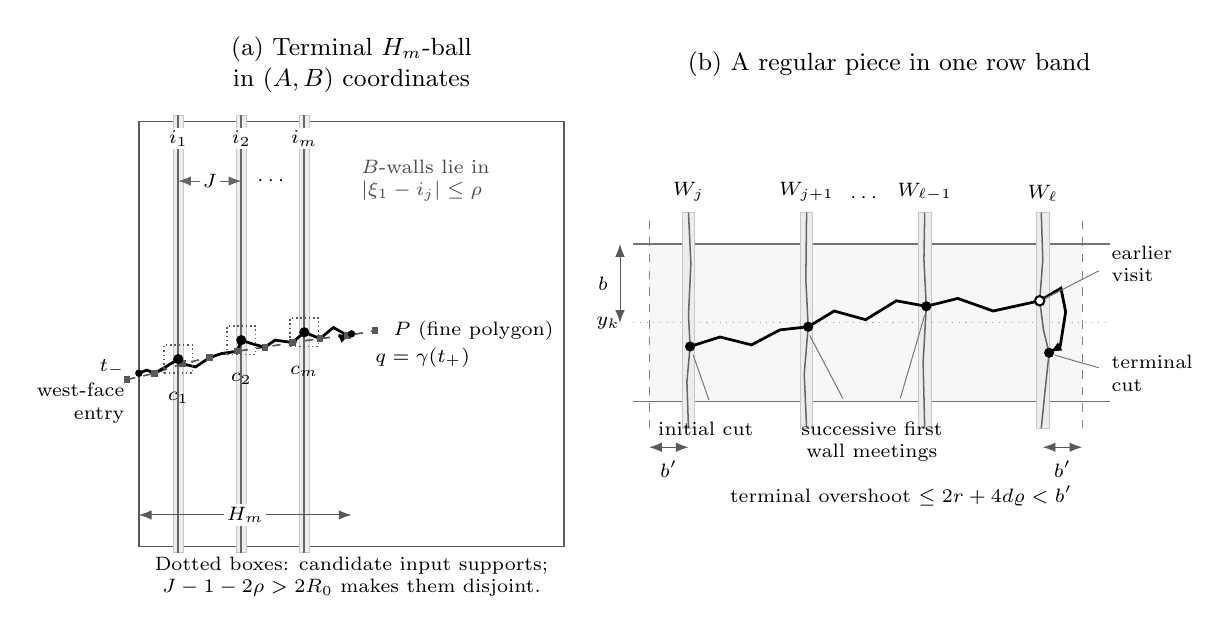
\begin{tikzpicture}[x=1cm,y=1cm,>=Latex,
  every node/.style={font=\scriptsize},
  path trace/.style={draw=black,line width=1pt},
  fine polygon/.style={draw=black!65,dashed,line width=.6pt},
  wall/.style={draw=black!60,line width=.55pt},
  wall strip/.style={fill=black!7,draw=black!22,line width=.3pt},
  support/.style={draw=black!65,densely dotted,line width=.55pt},
  cut/.style={circle,fill=black,inner sep=1.3pt}]

\begin{scope}[shift={(.42,.83)}]
  \node[font=\small,align=center] at (2.7,6.12)
    {(a) Terminal $H_m$-ball\\in $(A,B)$ coordinates};
  \draw[black!65,line width=.5pt] (0,0) rectangle (5.4,5.4);
  \foreach \v in {.5,1.3,2.1} {
    \path[wall strip] (\v-.06,-.08) rectangle (\v+.06,5.48);
    \draw[wall] (\v,-.08)--(\v,5.48);
  }
  \node[fill=white,inner sep=1pt] at (.5,5.18) {$i_1$};
  \node[fill=white,inner sep=1pt] at (1.3,5.18) {$i_2$};
  \node[fill=white,inner sep=1pt] at (2.1,5.18) {$i_m$};
  \draw[<->,black!60,line width=.35pt] (.5,4.64)--(1.3,4.64);
  \node[fill=white,inner sep=1pt] at (.9,4.64) {$J$};
  \node[fill=white,inner sep=1pt] at (1.7,4.64) {$\cdots$};
  \node[anchor=west,align=left,black!70] at (2.7,4.65)
    {$B$-walls lie in\\ $|\xi_1-i_j|\le\rho$};
  \draw[fine polygon]
    (-.15,2.12)--(.2,2.2)--(.55,2.32)--(.9,2.4)--(1.25,2.48)
    --(1.6,2.53)--(1.95,2.59)--(2.3,2.64)--(2.65,2.68)--(3,2.74);
  \draw[path trace,-{Latex[length=1.6mm]}]
    (0,2.2)--(.1,2.24)--(.2,2.2)--(.34,2.28)--(.5,2.38)--(.55,2.32)
    --(.72,2.28)--(.9,2.4)--(1.05,2.45)--(1.25,2.48)--(1.3,2.62)
    --(1.45,2.57)--(1.6,2.53)--(1.73,2.62)--(1.95,2.59)--(2.1,2.72)
    --(2.3,2.64)--(2.47,2.78)--(2.65,2.68)--(2.7,2.7);
  \foreach \px/\py in {-.15/2.12,.2/2.2,.55/2.32,.9/2.4,1.25/2.48,
                         1.6/2.53,1.95/2.59,2.3/2.64,2.65/2.68,3/2.74}
    \draw[fill=white,black!65,line width=.4pt]
      (\px-.035,\py-.035) rectangle (\px+.035,\py+.035);
  \foreach \px/\py in {.5/2.38,1.3/2.62,2.1/2.72} {
    \draw[support] (\px-.18,\py-.18) rectangle (\px+.18,\py+.18);
    \node[cut] at (\px,\py) {};
  }
  \fill (0,2.2) circle (1.35pt);
  \fill (2.7,2.7) circle (1.35pt);
  \node[anchor=east] at (-.06,2.27) {$t_-$};
  \node[anchor=east,align=right] at (-.06,1.82) {west-face\\ entry};
  \node[anchor=north] at (.5,2.08) {$c_1$};
  \node[anchor=north] at (1.3,2.32) {$c_2$};
  \node[anchor=north] at (2.1,2.42) {$c_m$};
  \node[anchor=west] at (3.11,2.74) {$P$ (fine polygon)};
  \node[anchor=west] at (2.88,2.4) {$q=\gamma(t_+)$};
  \draw[<->,black!65,line width=.35pt] (0,.4)--(2.7,.4);
  \node[fill=white,inner sep=1pt] at (1.35,.4) {$H_m$};
  \node[align=center] at (2.7,-.38)
    {Dotted boxes: candidate input supports;\\
     $J-1-2\rho>2R_0$ makes them disjoint.};
\end{scope}

\begin{scope}[shift={(6.7,1.67)}]
  \node[font=\small] at (3.25,5.28)
    {(b) A regular piece in one row band};
  \fill[black!3] (.2,1) rectangle (5.7,3);
  \draw[black!55,line width=.45pt] (0,1)--(6.05,1);
  \draw[black!55,line width=.45pt] (0,3)--(6.05,3);
  \draw[black!35,dotted,line width=.4pt] (0,2)--(6.05,2);
  \node[anchor=east] at (-.05,2) {$y_k$};
  \draw[<->,black!65,line width=.35pt] (-.17,2)--(-.17,3);
  \node[anchor=east] at (-.2,2.5) {$b$};
  \foreach \v in {.7,2.2,3.7,5.2}
    \path[wall strip] (\v-.08,.66) rectangle (\v+.08,3.4);
  \draw[wall] (.7,.66)--(.68,1.25)--(.72,1.7)--(.7,2.1)
    --(.73,2.75)--(.7,3.4);
  \draw[wall] (2.2,.66)--(2.17,1.35)--(2.22,1.95)--(2.19,2.55)
    --(2.2,3.4);
  \draw[wall] (3.7,.66)--(3.68,1.5)--(3.72,2.21)--(3.69,2.8)
    --(3.7,3.4);
  \draw[wall] (5.18,.66)--(5.24,1.25)--(5.28,1.62)--(5.21,1.9)
    --(5.16,2.28)--(5.2,2.8)--(5.18,3.4);
  \node[anchor=south] at (.7,3.42) {$W_j$};
  \node[anchor=south] at (2.2,3.42) {$W_{j+1}$};
  \node[anchor=south] at (3.7,3.42) {$W_{\ell-1}$};
  \node[anchor=south] at (5.2,3.42) {$W_\ell$};
  \node at (2.95,3.58) {$\cdots$};
  \draw[black!50,dashed,line width=.4pt] (.2,.66)--(.2,3.4);
  \draw[black!50,dashed,line width=.4pt] (5.7,.66)--(5.7,3.4);
  \draw[path trace,-{Latex[length=1.6mm]}]
    (.72,1.7)--(1.1,1.82)--(1.5,1.72)--(1.86,1.91)--(2.22,1.95)
    --(2.55,2.15)--(2.95,2.04)--(3.34,2.28)--(3.72,2.21)
    --(4.12,2.31)--(4.57,2.15)--(5.16,2.28)--(5.43,2.44)
    --(5.49,2.14)--(5.42,1.7)--(5.28,1.62);
  \foreach \px/\py in {.72/1.7,2.22/1.95,3.72/2.21,5.28/1.62}
    \node[cut] at (\px,\py) {};
  \draw[fill=white,line width=.75pt] (5.16,2.28) circle (1.7pt);
  \node[anchor=north,align=center] at (.92,.86) {initial cut};
  \draw[black!55,line width=.35pt] (.96,1.02)--(.76,1.59);
  \node[anchor=north,align=center] at (3.03,.86)
    {successive first\\ wall meetings};
  \draw[black!55,line width=.35pt] (2.66,1.04)--(2.24,1.84);
  \draw[black!55,line width=.35pt] (3.39,1.04)--(3.7,2.1);
  \node[anchor=west,align=left] at (5.95,2.75) {earlier\\ visit};
  \draw[black!55,line width=.35pt] (5.91,2.66)--(5.23,2.31);
  \node[anchor=west,align=left] at (5.95,1.36) {terminal\\ cut};
  \draw[black!55,line width=.35pt] (5.91,1.43)--(5.35,1.59);
  \draw[<->,black!65,line width=.35pt] (.2,.42)--(.7,.42);
  \draw[<->,black!65,line width=.35pt] (5.2,.42)--(5.7,.42);
  \node[anchor=north] at (.45,.37) {$b'$};
  \node[anchor=north] at (5.45,.37) {$b'$};
  \node[align=center] at (3.4,-.2)
    {terminal overshoot $\le 2r+4d\varrho<b'$};
\end{scope}
\end{tikzpicture}
\end{document}
